% This is a Basic Assignment Paper but with like Code and stuff allowed in it. 

\documentclass[11pt]{article}

% Preamble

\usepackage[margin=1in]{geometry}
\usepackage{amsfonts, amsmath, amssymb}
\usepackage{fancyhdr, float, graphicx}
\usepackage[utf8]{inputenc} % Required for inputting international characters
\usepackage[T1]{fontenc} % Output font encoding for international characters
\usepackage{fouriernc} % Use the New Century Schoolbook font
\usepackage[nottoc, notlot, notlof]{tocbibind}
\usepackage{listings}
\usepackage{xcolor}
\usepackage{float}

\definecolor{codegreen}{rgb}{0,0.6,0}
\definecolor{codegray}{rgb}{0.5,0.5,0.5}
\definecolor{codepurple}{rgb}{0.58,0,0.82}
\definecolor{backcolour}{rgb}{0.95,0.95,0.92}

\lstdefinestyle{mystyle}{
    backgroundcolor=\color{backcolour},   
    commentstyle=\color{codegreen},
    keywordstyle=\color{magenta},
    numberstyle=\tiny\color{codegray},
    stringstyle=\color{codepurple},
    basicstyle=\ttfamily\footnotesize,
    breakatwhitespace=false,         
    breaklines=true,                 
    captionpos=b,                    
    keepspaces=true,                 
    numbers=left,                    
    numbersep=5pt,                  
    showspaces=false,                
    showstringspaces=false,
    showtabs=false,                  
    tabsize=2
}

\lstset{style=mystyle}

% Header and Footer
\pagestyle{fancy}
\fancyhead{}
\fancyfoot{}
\fancyhead[L]{\textit{\Large{Computer Networks Assignment 10}}}
%\fancyhead[R]{\textit{something}}
\fancyfoot[C]{\thepage}
\renewcommand{\footrulewidth}{1pt}



% Other Doc Editing
% \parindent 0ex
%\renewcommand{\baselinestretch}{1.5}

\begin{document}
	
	\begin{titlepage} 
		\centering 
		
		%---------------------------NAMES-------------------------------
		
		\huge\textsc{
			MIT World Peace University
		}\\
	
		\vspace{0.75\baselineskip} % space after Uni Name
		
		\LARGE{
			Computer Networks\\
			Second Year B. Tech, Semester 3
		}
		
		\vfill % space after Sub Name
		
		%--------------------------TITLE-------------------------------
		
		\rule{\textwidth}{1.6pt}\vspace*{-\baselineskip}\vspace*{2pt}
		\rule{\textwidth}{0.6pt}
		\vspace{0.75\baselineskip} % Whitespace above the title
		
		
		
		\huge{\textsc{
			DHCP, DNS and Web Server configuration
			}} \\
		
		
		
		\vspace{0.5\baselineskip} % Whitespace below the title
		\rule{\textwidth}{0.6pt}\vspace*{-\baselineskip}\vspace*{2.8pt}
		\rule{\textwidth}{1.6pt}
		
		\vspace{1\baselineskip} % Whitespace after the title block

		%--------------------------SUBTITLE --------------------------	
			
		\LARGE\textsc{
			Practical Report\\
			Assignment 10
		} % Subtitle or further description
		\vfill
		
		%--------------------------AUTHOR-------------------------------
		
		Prepared By
		\vspace{0.5\baselineskip} % Whitespace before the editors
		
		\Large{
			Krishnaraj Thadesar \\
			Cyber Security and Forensics\\
			Batch A1, PA 20
		}
		
		
		\vspace{0.5\baselineskip} % Whitespace below the editor list
		\today

	\end{titlepage}
	
	
\tableofcontents
\thispagestyle{empty}
\clearpage


\setcounter{page}{1}

\section{Aim and Objectives}
\subsection*{Aim}
To Configure network using Dynamic Host Configuration Protocol (DHCP), DNS and Web server Use Ping utility to test connectivity.
\subsection*{Objectives}
\begin{enumerate}
	\item To learn the DHCP installation and understand the practical use of DHCP, DNS and Web server.
	\item To learn the mechanism to access the remote machine by using ping utility to test connectivity.
\end{enumerate}
\section{Devices}

\subsection{Devices Used}
\begin{enumerate}
	\item 1 Wireless Router WRT300N
	\item 1 Switch 2950
	\item 5 Generic PCs
	\item 3 Laptops
	\item 1 Web Server
\end{enumerate}

\subsection{Device Info and IP Addresses}

Subnet Mask: 255.255.255.0

\begin{table}[H] 
	\centering
	\begin{tabular}{|c|c|c|}
	\hline
	\textbf{Name} & \textbf{Type}      & \textbf{IP}    \\ 
	\hline
	PC0           & PC                 & 192.168.10.1   \\ 
	\hline
	PC1           & PC                 & 192.168.10.2   \\ 
	\hline
	PC2           & PC                 & 192.168.10.3   \\ 
	\hline
	PC3           & PC                 & 192.168.10.4   \\ 
	\hline
	PC6           & PC                 & 192.168.10.5   \\ 
	\hline
	PC5           & PC                 & 192.168.10.6   \\ 
	\hline
	Laptop0       & Laptop             & 192.168.10.7   \\ 
	\hline
	Laptop1       & Laptop             & 192.168.10.8   \\ 
	\hline
	Laptop2       & Laptop             & 192.168.10.9   \\ 
	\hline
	Laptop3       & Laptop             & 192.168.10.10  \\ 
	\hline
	Switch0       & 2950-24
					Switch & None           \\ 
	\hline
	Switch1       & 2950-24
					Switch & None           \\ 
	\hline
	Switch2       & Generic
					Switch & None           \\
	\hline
	\end{tabular}
	\end{table}

\section{Cables}
\begin{enumerate}
	\item Straight LAN Cable to connect unlike Devices
	\item Crossover LAN Cable to connect like Devices
\end{enumerate}

\section{Commands}
\begin{verbatim}
Router>enable
Router#config terminal
Router(config)#int fa0/0
Router(config-if)#ip add 192.168.1.1 255.255.255.0
Router(config-if)#no shutdown
Router(config-if)#exit
Router(config)#
Router(config)#ip dhcp pool MY_LAN
Router(dhcp-config)#network 192.168.1.0 255.255.255.0
Router(dhcp-config)#default-router 192.168.1.1
Router(dhcp-config)#dns-server 192.168.1.10
\end{verbatim}

\section{Procedure to Configure LAN}
\begin{enumerate}
	\item Create The network topology on the Packet tracer, that has a router, a few PCS near the router, and some connected to it via LAN cables. 
	\item Add a Web server which is connected to a switch that is connected to other end devices. 
	\item Run the commands on the router to configure it. 
	\item Go to the GUI tab in the router, and select the Wireless tab, where you can go to wireless security, and select security mode to WPA2, personal, and encryption to AE5. Assign a password. 
	\item To the PCs not connected to the router directly, install a wireless network card in them after turning them off, and then turn them back on. 
	\item Go the PC wireless in the Desktop Settings, and navigate to the Connect Tab. Here refersh the network, and add the WPA2 Passkey that you have assigned to the router. 
	\item To the webserver, add a Fast ethernet port to connect it. 
	\item Configure the Web Server, and add the Default gateway as 10.0.0.1
	\item Go to the services tab in the web server, and in DHCP, turn it on, and configure the starting and the ending IP addresses. Save. 
	\item Assign IP Addresses to all the other computers, by selecting on the DHCP Radiobutton instead of the static one, and wait for it to query and assign the IP. Ping and check. 
\end{enumerate}

\section{Platform}
	\textbf{Operating System}: Arch Linux x86-64\\
	\textbf{IDEs or Text Editors Used}: Visual Studio Code\\
	\textbf{Programs Used}: Cisco Packet Tracer v8.2

\section{Connection Screenshot}

\begin{figure}[H]
	\centering
	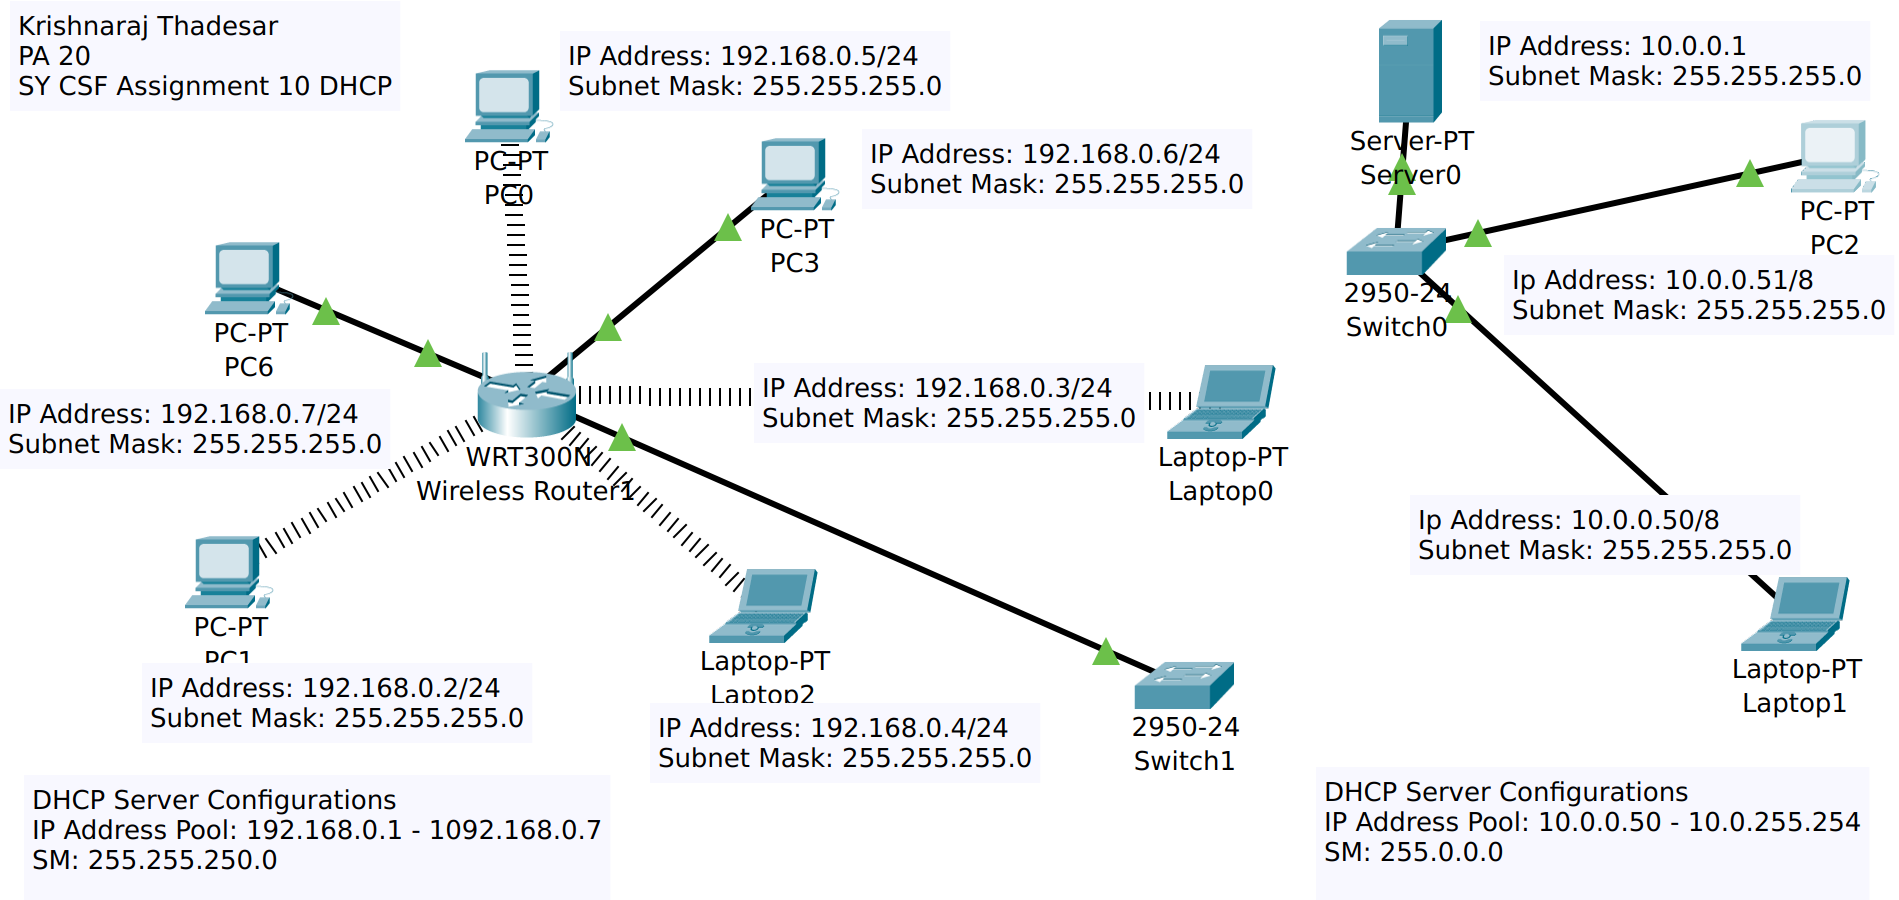
\includegraphics[scale=0.35]{../Screenshots/Assignment_10_screenshot.png}
\end{figure}


\section{Conclusion}
DHCP, DNS and Web Server configurations were implemented and understood successfully. 
\end{document}